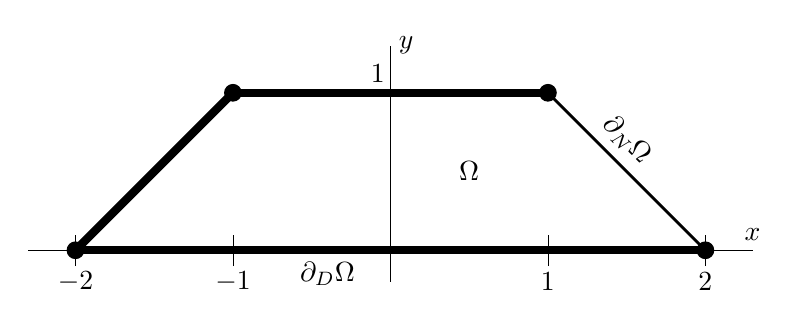
\begin{tikzpicture}[scale=2.000000]
% originally created, in part, by script tri2tikz.py command line:
%   tri2tikz.py --polyonly --nodesize 1.0 --scale 2.0 ../c/ch8/meshes/trap tmp/trap.tikz
% with by-hand edits
  \draw[thin] (0.0,-0.2) -- (0.0,1.3);
  \draw[thin] (-2.3,0.0) -- (2.3,0.0);
  \node at (2.3,0.1) {$x$};
  \node at (0.1,1.3) {$y$};
  \node at (0.5,0.5) {$\Omega$};
  \node at (-0.08,1.12) {$1$};
  \draw[very thin] (-2.0,-0.1) -- (-2.0,0.1);
  \node at (-2.0,-0.2) {$-2$};
  \draw[very thin] (-1.0,-0.1) -- (-1.0,0.1);
  \node at (-1.0,-0.2) {$-1$};
  \draw[very thin] (1.0,-0.1) -- (1.0,0.1);
  \node at (1.0,-0.2) {$1$};
  \draw[very thin] (2.0,-0.1) -- (2.0,0.1);
  \node at (2.0,-0.2) {$2$};
  \node at (-0.4,-0.15) {$\partial_D \Omega$};
  \node[rotate=-45] at (1.5,0.7) {$\partial_N \Omega$};
  \draw[line width=1.0pt] (2.000000,0.000000) -- (1.000000,1.000000);
  \draw[line width=3.0pt] (1.000000,1.000000) -- (-1.000000,1.000000);
  \draw[line width=3.0pt] (-1.000000,1.000000) -- (-2.000000,0.000000);
  \draw[line width=3.0pt] (-2.000000,0.000000) -- (2.000000,0.000000);
  \filldraw (2.0,0.0) circle (1.5pt);
  \filldraw (1.0,1.0) circle (1.5pt);
  \filldraw (-1.0,1.0) circle (1.5pt);
  \filldraw (-2.0,0.0) circle (1.5pt);
\end{tikzpicture}
